\documentclass[12pt, xcolor=table]{beamer}

\usepackage{geometry}

\usepackage{lmodern}
\usepackage[utf8]{inputenc}
\usepackage[T1]{fontenc}		
\usepackage[english]{babel}

\usepackage{siunitx}

\usepackage{xcolor, colortbl}
\definecolor{darkgreen}{RGB}{0, 155, 85}
\definecolor{elancourt}{rgb}{1,.79,.5}
\definecolor{paris}{rgb}{.84,.1,.11}
\definecolor{nantes}{rgb}{.17,.51,.73}

\renewcommand<>\cellcolor[1]{\only#2{\beameroriginal\cellcolor{#1}}}

\definecolor{LOSS35}{RGB}{255,0,0}
\definecolor{LOSS1535}{RGB}{255,122,12}
\definecolor{LOSS0515}{RGB}{255,181,12}
\definecolor{STBL}{RGB}{58,255,12}
\definecolor{GAIN0515}{RGB}{58,178,12}
\definecolor{GAIN1535}{RGB}{56,136,17}
\definecolor{GAIN35}{RGB}{50,119,16}


\usepackage{graphicx}
\usepackage{floatrow}
\usepackage[
    scriptsize,
    labelformat=empty
]{caption}

\usepackage{enumitem}

\usepackage{standalone}

\usepackage{multirow}

\usepackage{array}
\newcolumntype{x}[1]{>{\centering\let\newline\\\arraybackslash\hspace{0pt}}m{#1}}
\usepackage{booktabs}
\usepackage{makecell}

\usepackage{tikz}
\usetikzlibrary{calc, 3d, shadows, decorations, shapes, fadings, trees, backgrounds, fit}
\usepackage{pgfplots}
\usepackage{pgfplotstable}
\usepackage{forest}
\usepackage[final]{animate}

\usepackage{amsmath}
\usepackage{amsthm}
\usepackage{amsfonts}
\usepackage{amssymb}
\usepackage{mathrsfs}
\usepackage{bm}
\usepackage{bbold}
\usepackage{stmaryrd}
\usepackage{mleftright}
    
\usepackage[
    backend=biber,
    style=authoryear,
    dashed=false,
    sorting=nty,
    maxbibnames=5,
    minbibnames=5,
    maxcitenames=1,
    uniquelist=false,
    uniquename=false,
    hyperref=true,
    backref=true,
    backrefstyle=all+,
    isbn=false,
    url=false,
    doi=false
]{biblatex}
\usepackage{xpatch}

\addbibresource{references.bib}

\usepackage[acronym, toc, automake=true]{glossaries}

\usepackage{hyperref}
\hypersetup{
    pdftitle={Semantic aware quality evaluation of 3D building models},
    pdfauthor={Oussama Ennafii},
    pdfkeywords={3D urban modeling} {buildings} {quality assessment} {taxonomy} {classification} {error detection} {geometry} {aerial imagery} {Very High Spatial Resolution} {Digital Surface Model},
    pdfstartview={FitH},
    unicode=true
}

\setbeamerfont{footnote}{size=\tiny}

\tikzset{
    invisible/.style={opacity=0},
    visible on/.style={alt=#1{}{invisible}},
    alt/.code args={<#1>#2#3}{
        \alt<#1>{\pgfkeysalso{#2}}{\pgfkeysalso{#3}}
    },
}

\NewDocumentCommand{\evalat}{sO{\big}mm}{%
    \IfBooleanTF{#1}
    {\mleft. #3 \mright|_{#4}}
    {#3#2|_{#4}}%
}
\makeatletter
\newcommand{\ostar}{\mathbin{\mathpalette\make@circled\star}}
\newcommand{\make@circled}[2]{%
    \ooalign{$\m@th#1\smallbigcirc{#1}$\cr\hidewidth$\m@th#1#2$\hidewidth\cr}%
}
\newcommand{\smallbigcirc}[1]{%
    \vcenter{\hbox{\scalebox{0.77778}{$\m@th#1\bigcirc$}}}%
}
\makeatother


\usepackage[useregional]{datetime2}

\usepackage{style/glossaries}

\usetheme{ign}

\title{Semantic aware quality evaluation of 3D building models}
\subtitle{A scalable approach}
\date{\tiny \DTMdisplaydate{2020}{1}{10}{5}}
\author{
    Oussama Ennafii
}

\institute{
    PhD defense
}

\begin{document}
    \begin{frame}[plain]
        \titlepage
    \end{frame}

    \section{Introduction}
        \subsection{Context}
            \begin{frame}{Applications of \texorpdfstring{\acrshort*{acr::3d}}{3D} models}
                \framesubtitle<1>{Physical simulation}
                \framesubtitle<2>{Urban planning}
                \framesubtitle<3>{Entertainement}

                \temporal<2>{
                    \begin{figure}[H]
                        \centering
                        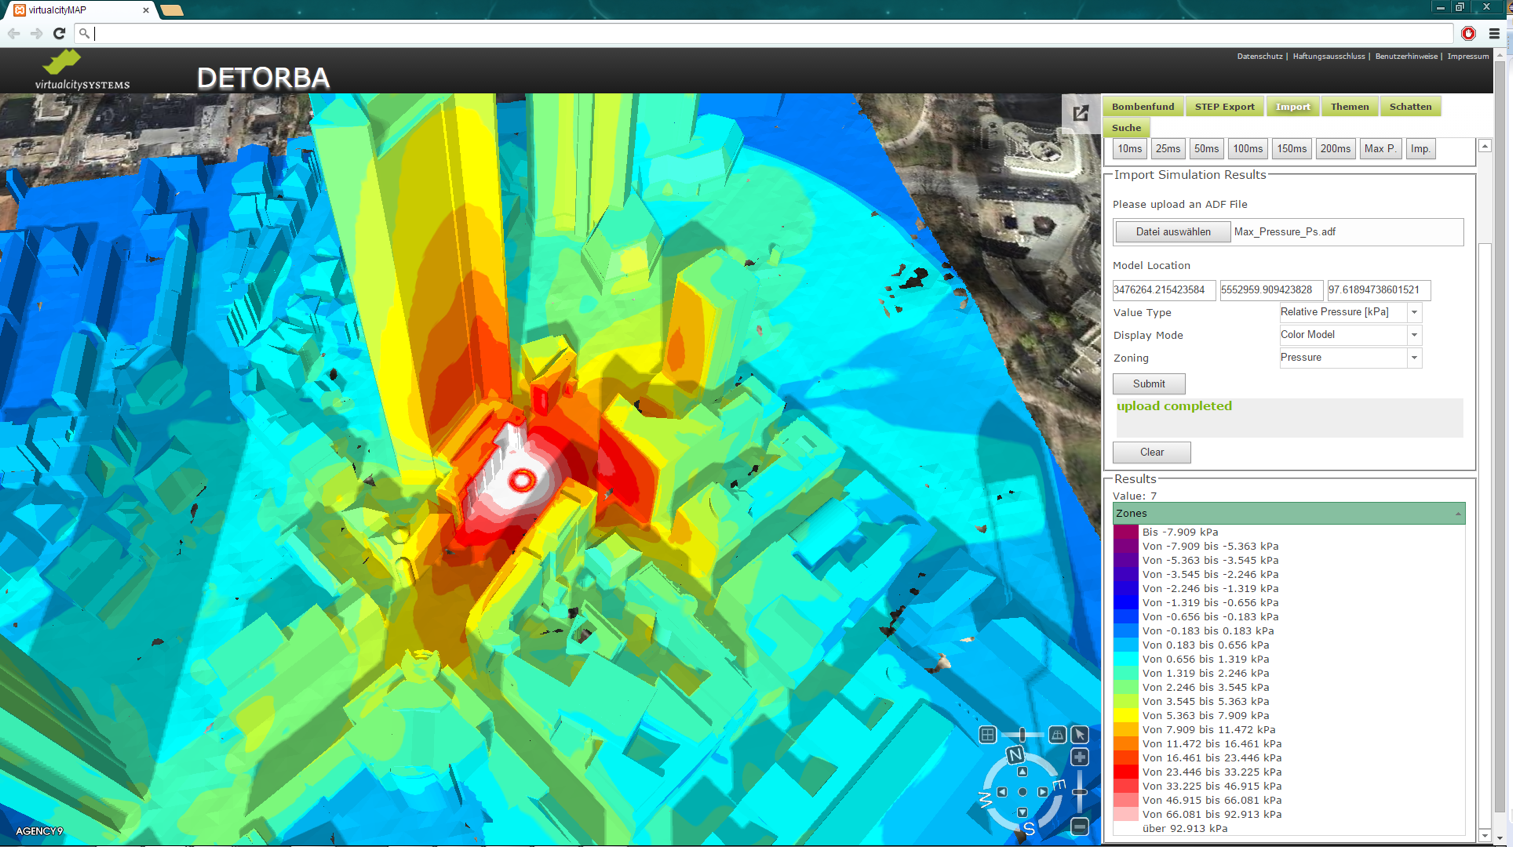
\includegraphics[width=.8\textwidth]{images/introduction/3d_model_applications/explosion_simulation}
                        \caption{Explosion simulation~\parencite{biljecki2015applications}.}
                    \end{figure}
                }
                {
                    \begin{figure}[H]
                        \centering
                        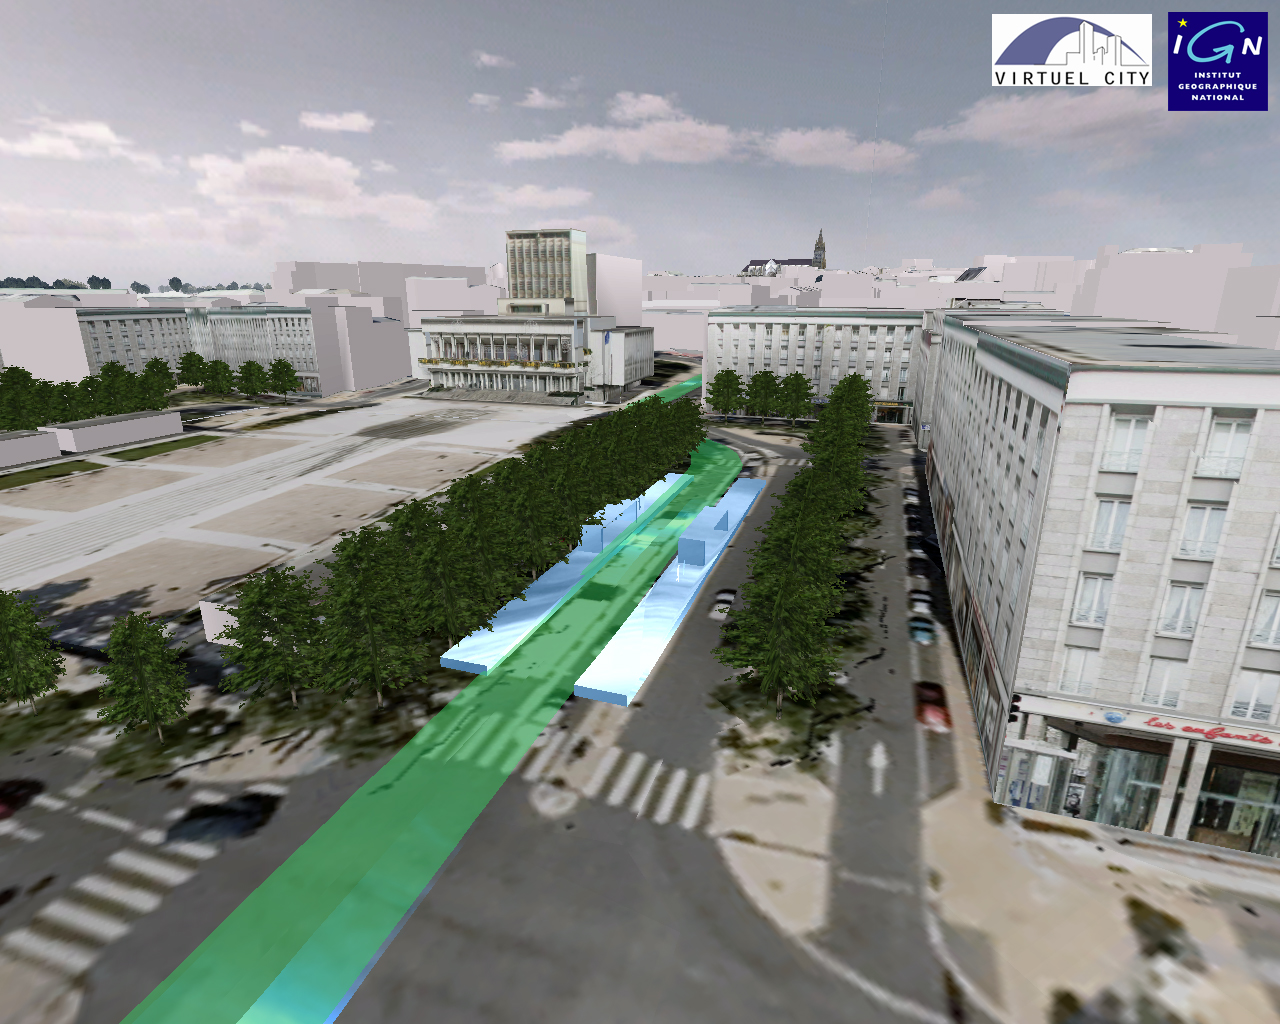
\includegraphics[width=.8\textwidth]{images/introduction/3d_model_applications/brest_tramway}
                        \caption{Example of the use of city \gls{acr::3d} models in public consultation in Brest.}
                    \end{figure}
                }
                {
                    \begin{figure}[H]
                        \centering
                        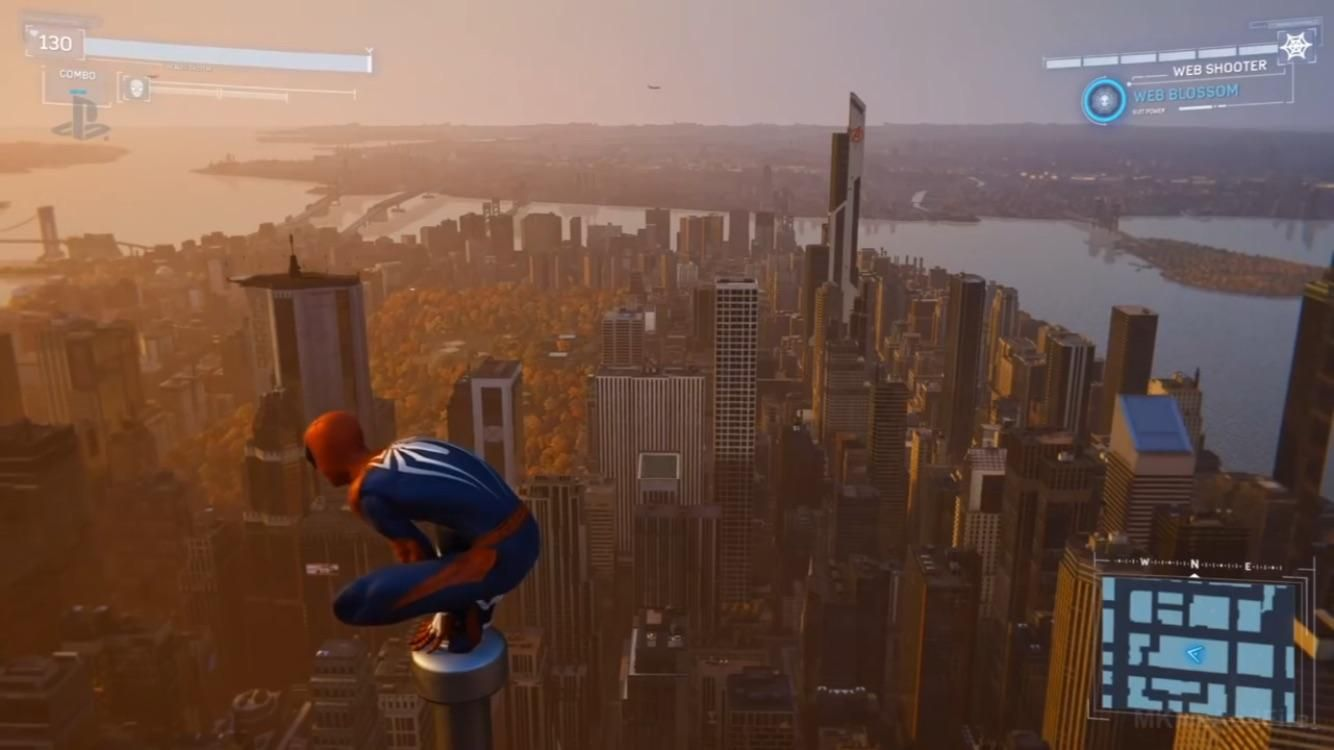
\includegraphics[width=.8\textwidth]{images/introduction/3d_model_applications/spider_man}
                        \caption{Example of the use of city \gls{acr::3d} models in video games.}
                    \end{figure}
                }
            \end{frame}

            \begin{frame}{Modeling or reconstruction}
                \begin{columns}[T]
                    \centering
                    \begin{column}{.5\textwidth}
                        \includestandalone[mode=buildnew, width=\textwidth]{figures/model_vs_mesh/mesh_model}
                        \footnotesize
                        \begin{itemize}[label=\(\blacktriangleright\), font=\color{IGNGreen}]
                            \item<1-> Building surface \underline{reconstruction}.
                            \item<2-> Geometric \underline{fidelity}.
                            \item<3-> \num{10000} facets.
                            \item<4-> Weak geometric constraints.
                        \end{itemize}
                    \end{column}
                    \begin{column}{.5\textwidth}
                        \includestandalone[mode=buildnew, width=\textwidth]{figures/model_vs_mesh/ground_truth_model_animated}
                        \footnotesize
                        \begin{itemize}[label=\(\blacktriangleright\), font=\color{IGNGreen}]
                            \item<1-> Building \underline{modeling}.
                            \item<2-> Geometric fidelity + Compacity.
                            \item<3-> \num{800} facets.
                            \item<only@4> Semantics \(\implies\) impact on geometry.
                            \item<only@5> \textit{Implicit} semantics. \phantom{on geometry}
                        \end{itemize}
                    \end{column}
                \end{columns}
            \end{frame}

            \begin{frame}{\texorpdfstring{\acrshort*{acr::3d}}{3D} model}
                \centering
                \includestandalone[mode=buildnew, width=.7\textwidth]{figures/model_information}
                
            \end{frame}

            \begin{frame}{\texorpdfstring{\acrshort*{acr::3d}}{3D} building modeling}
                \begin{figure}[H]
                    \centering
                    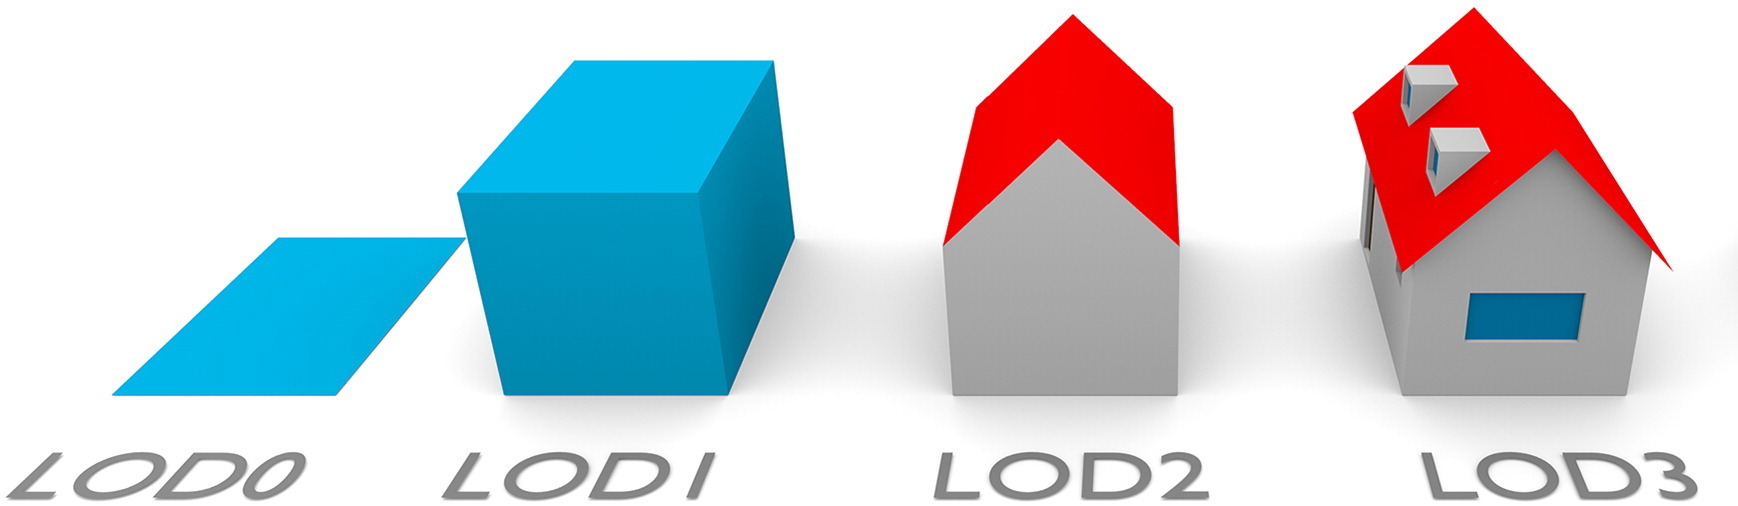
\includegraphics[width=\textwidth]{images/introduction/lods_3}
                    \caption{\glspl{acr::lod} considered in the study~\parencite{biljecki2016improved}.}
                \end{figure}
            \end{frame}
        
        \subsection{Quality evaluation}
            \begin{frame}{Modeling errors}{Different point of views}
                \begin{itemize}[label=\(\blacktriangleright\), font=\color{IGNGreen}]
                    \item<1-> Errors in format: compliancy to OGC standard\footfullcite{ledoux2013validation}.
                    \item<2-> Errors in surface reconstruction\footfullcite{berger2013benchmark}.
                    \item<3-> Errors in Modeling\footfullcite{rottensteiner2012isprs}.
                \end{itemize}
            \end{frame}

            \begin{frame}{Need for semantics}
                \begin{itemize}[label=\(\blacktriangleright\), font=\color{IGNGreen}]
                    \item<1-> Modeling \(\longleftrightarrow\) compromise between:
                    \begin{itemize}[label=\(\blacktriangleright\), font=\color{IGNGreen}]
                        \item<2-> geometric accuracy;
                        \item<3-> and \textit{implicit} semantics.
                    \end{itemize}
                    \item<4-> Errors are \underline{geometric} and \underline{semantic} in nature.
                \end{itemize}
            \end{frame}

            \begin{frame}{Goal}
                \begin{itemize}[label=\(\blacktriangleright\), font=\color{IGNGreen}]
                    \item<1-> \underline{Define errors} that affects building \gls{acr::3d} models.
                    \item<2-> Design a method for \underline{error detection}.
                \end{itemize}
            \end{frame}

            \begin{frame}{Challenges}
                \begin{itemize}[label=\(\blacktriangleright\), font=\color{IGNGreen}]
                    \item<1-> Reference data are \underline{expensive}.
                    \item<2-> Large scale : small city level > \underline{\num{1000}} buildings.
                    \item<3-> \underline{Different} urban scenes \(\implies\) High \underline{heterogeneity}.
                    \item<6-> Manual evaluation: \SI[per-mode=repeated-symbol]{2}{\hour\per\km\squared\per\expert}.
                \end{itemize}
            \end{frame}
            
            \begin{frame}{State of the art}
                \centering
                \includestandalone[mode=buildnew, width=\textwidth]{figures/state_of_the_art}
            \end{frame}

            \begin{frame}{What do we want?}
                \begin{itemize}[label=\(\blacktriangleright\), font=\color{IGNGreen}, itemsep=1em]
                    \item<1-> Readily accessible reference data;
                    \item<2-> \textbf{Scalability} up to city level;
                    \item<3-> Genericity towards:
                        \begin{enumerate}[label=(\roman*)]
                            \item<4-> modeling approach;
                            \item<5-> urban scene.
                        \end{enumerate}
                    \item<6-> \textbf{Automation}: low human intervention.
                \end{itemize}
            \end{frame}

            \begin{frame}{Our answer}
                \begin{enumerate}[label=\arabic* --, itemsep=2em, font=\color{IGNGreen}]
                    \item<1-> Semantic error taxonomy;
                    \item<2-> Learning based evaluation approach;
                    \item<3-> Experimental validation.
                \end{enumerate}
            \end{frame}

    \section{Semantic evaluation}
        \begin{frame}{The issue at hand}
            \begin{itemize}[label=\(\blacktriangleright\), font=\color{IGNGreen}, itemsep=2em]
                \item<1-> Large scale (coverage) \(\implies\) Errors independent from:
                \begin{itemize}
                    \item<2-> Urban scene;
                    \item<3-> Modeling approach.
                \end{itemize}
            \end{itemize}
        \end{frame}

        \subsection{General layout}
            \begin{frame}{Hierarchization and Modularity}
                \begin{itemize}[label=\(\blacktriangleright\), font=\color{IGNGreen}, itemsep=2em]
                    \item<1-> Hierarchization:
                        \begin{itemize}[label=\(\blacktriangleright\), font=\color{IGNGreen}]
                            \item<2-> \underline{Iteratively} define more and more specific errors;
                            \item<3-> Each \underline{specificity level}: errors as general as possible;
                            \item<4-> \texttt{finesse} = specificity level.
                        \end{itemize}
                    \item<4-> Modularity:
                        \begin{itemize}[label=\(\blacktriangleright\), font=\color{IGNGreen}]
                            \item<5-> An error \(\equiv\) Composition of \underline{basic errors} common to all scenes.
                        \end{itemize}
                \end{itemize}
            \end{frame}
        
            \begin{frame}{Error classification}
                \includestandalone[mode=buildnew, width=\textwidth]{figures/taxonomy_tree_animated}
            \end{frame}

        \subsection{Roof modeling case}
            \begin{frame}{Atomic errors}{\texorpdfstring{\acrshort*{acr::2d}}{2D} errors}
                \begin{itemize}[label=\(\blacktriangleright\), font=\color{IGNGreen}]
                    \item<1-> \Acrfull{acr::2d} errors:
                    \begin{itemize}[label=\(\blacktriangleright\), font=\color{IGNGreen}]
                        \item<2-> Segmentation issue (semantic):
                        \begin{itemize}
                            \item<3-4> Under segmentation;
                        \end{itemize}
                    \end{itemize}
                \end{itemize}
                \begin{overlayarea}{\textwidth}{.5\textheight}
                    \only<3->{
                        \begin{columns}[T]
                            \begin{column}{.5\textwidth}
                                \centering
                                \begin{figure}[H]
                                    \centering
                                    \alt<3>{
                                        \includestandalone[mode=buildnew, height=.4\textheight]{figures/errors/building/bos}
                                    }{
                                        \includestandalone[mode=buildnew, height=.4\textheight]{figures/errors/facet/correct_fos_fus_fib_fig}
                                    }
                                    \caption{
                                        Ground truth buildings.
                                    }
                                \end{figure}
                            \end{column}
                            \begin{column}{.5\textwidth}
                                \begin{figure}[H]
                                    \centering
                                    \alt<3>{
                                        \includestandalone[mode=buildnew, height=.4\textheight]{figures/errors/building/bus}
                                    }{
                                        \includestandalone[mode=buildnew, height=.4\textheight]{figures/errors/facet/fus}
                                    }
                                    \caption{
                                        Model.
                                    }
                                \end{figure}
                            \end{column}
                        \end{columns}
                    }
                \end{overlayarea}
            \end{frame}

            \begin{frame}{Atomic errors}{\texorpdfstring{\acrshort*{acr::2d}}{2D} errors}
                \begin{itemize}[label=\(\blacktriangleright\), font=\color{IGNGreen}]
                    \item<1-> \Acrfull{acr::2d} errors:
                    \begin{itemize}[label=\(\blacktriangleright\), font=\color{IGNGreen}]
                        \item<2-> Segmentation issue (semantic):
                        \begin{itemize}
                            \item<3-4> Over segmentation.
                        \end{itemize}
                    \end{itemize}
                \end{itemize}
                \begin{overlayarea}{\textwidth}{.5\textheight}
                    \only<3->{
                        \begin{columns}[T]
                            \begin{column}{.5\textwidth}
                                \centering
                                \begin{figure}[H]
                                    \centering
                                    \alt<3>{
                                        \includestandalone[mode=buildnew, height=.4\textheight]{figures/errors/building/bus}
                                    }{
                                        \includestandalone[mode=buildnew, height=.4\textheight]{figures/errors/facet/correct_fos_fus_fib_fig}
                                    }
                                    \caption{
                                        Ground truth buildings.
                                    }
                                \end{figure}
                            \end{column}
                            \begin{column}{.5\textwidth}
                                \begin{figure}[H]
                                    \centering
                                    \alt<3>{
                                        \includestandalone[mode=buildnew, height=.4\textheight]{figures/errors/building/bos}
                                    }{
                                        \includestandalone[mode=buildnew, height=.4\textheight]{figures/errors/facet/fos}
                                    }
                                    \caption{
                                        Model.
                                    }
                                \end{figure}
                            \end{column}
                        \end{columns}
                    }
                \end{overlayarea}
            \end{frame}

            \begin{frame}{Atomic errors}{\texorpdfstring{\acrshort*{acr::2d}}{2D} errors}
                \begin{itemize}[label=\(\blacktriangleright\), font=\color{IGNGreen}]
                    \item<1-> \Acrfull{acr::2d} errors:
                    \begin{itemize}[label=\(\blacktriangleright\), font=\color{IGNGreen}]
                        \item<2-> Border issue (geometric):
                        \begin{itemize}
                            \item<3-4> Inaccurate topology;
                        \end{itemize}
                    \end{itemize}
                \end{itemize}
                \begin{overlayarea}{\textwidth}{.5\textheight}
                    \only<3->{
                        \begin{columns}[T]
                            \begin{column}{.5\textwidth}
                                \centering
                                \begin{figure}[H]
                                    \centering
                                    \alt<3>{
                                        \includestandalone[mode=buildnew, height=.4\textheight]{figures/errors/building/correct_bit}
                                    }{
                                        \includestandalone[mode=buildnew, height=.4\textheight]{figures/errors/facet/correct_fit}
                                    }
                                    \caption{
                                        Ground truth buildings.
                                    }
                                \end{figure}
                            \end{column}
                            \begin{column}{.5\textwidth}
                                \begin{figure}[H]
                                    \centering
                                    \alt<3>{
                                        \includestandalone[mode=buildnew, height=.4\textheight]{figures/errors/building/bit}
                                    }{
                                        \includestandalone[mode=buildnew, height=.4\textheight]{figures/errors/facet/fit}
                                    }
                                    \caption{
                                        Model.
                                    }
                                \end{figure}
                            \end{column}
                        \end{columns}
                    }
                \end{overlayarea}
            \end{frame}

            \begin{frame}{Atomic errors}{\texorpdfstring{\acrshort*{acr::2d}}{2D} errors}
                \begin{itemize}[label=\(\blacktriangleright\), font=\color{IGNGreen}]
                    \item<1-> \Acrfull{acr::2d} errors:
                    \begin{itemize}[label=\(\blacktriangleright\), font=\color{IGNGreen}]
                        \item<2-> Border issue (geometric):
                        \begin{itemize}
                            \item<3-4> Imprecise border.
                        \end{itemize}
                    \end{itemize}
                \end{itemize}
                \begin{overlayarea}{\textwidth}{.5\textheight}
                    \only<3->{
                        \begin{columns}[T]
                            \begin{column}{.5\textwidth}
                                \centering
                                \begin{figure}[H]
                                    \centering
                                    \alt<3>{
                                        \includestandalone[mode=buildnew, height=.4\textheight]{figures/errors/building/correct_bib}
                                    }{
                                        \includestandalone[mode=buildnew, height=.4\textheight]{figures/errors/facet/correct_fos_fus_fib_fig}
                                    }
                                    \caption{
                                        Ground truth buildings.
                                    }
                                \end{figure}
                            \end{column}
                            \begin{column}{.5\textwidth}
                                \begin{figure}[H]
                                    \centering
                                    \alt<3>{
                                        \includestandalone[mode=buildnew, height=.4\textheight]{figures/errors/building/bib}
                                    }{
                                        \includestandalone[mode=buildnew, height=.4\textheight]{figures/errors/facet/fib}
                                    }
                                    \caption{
                                        Model.
                                    }
                                \end{figure}
                            \end{column}
                        \end{columns}
                    }
                \end{overlayarea}
            \end{frame}

            \begin{frame}{Atomic errors}{\texorpdfstring{\acrshort*{acr::3d}}{3D} errors}
                \begin{itemize}[label=\(\blacktriangleright\), font=\color{IGNGreen}]
                    \item<1-> \Acrfull{acr::3d} errors:
                    \begin{itemize}[label=\(\blacktriangleright\), font=\color{IGNGreen}]
                        \item<2-3> Imprecise geometry.
                        \begin{itemize}
                            \item 
                        \end{itemize}
                    \end{itemize}
                \end{itemize}
                \begin{overlayarea}{\textwidth}{.5\textheight}
                    \only<3->{
                        \begin{columns}[T]
                            \begin{column}{.5\textwidth}
                                \centering
                                \begin{figure}[H]
                                    \centering
                                    \alt<3>{
                                        \includestandalone[mode=buildnew, height=.4\textheight]{figures/errors/building/correct_big}
                                    }{
                                        \includestandalone[mode=buildnew, height=.4\textheight]{figures/errors/facet/correct_fos_fus_fib_fig}
                                    }
                                    \caption{
                                        Ground truth buildings.
                                    }
                                \end{figure}
                            \end{column}
                            \begin{column}{.5\textwidth}
                                \begin{figure}[H]
                                    \centering
                                    \alt<3>{
                                        \includestandalone[mode=buildnew, height=.4\textheight]{figures/errors/building/big}
                                    }{
                                        \includestandalone[mode=buildnew, height=.4\textheight]{figures/errors/facet/fig}
                                    }
                                    \caption{
                                        Model.
                                    }
                                \end{figure}
                            \end{column}
                        \end{columns}
                    }
                \end{overlayarea}
            \end{frame}

    \section{Learning based evaluation}
        \begin{frame}{Evaluation as classification}
            \begin{itemize}[label=$\blacktriangleright$, font=\color{IGNGreen}]
                \item<1-> Error detection \(\longleftrightarrow\) supervized classification:
                \begin{itemize}[label=---]
                    \item<2-> Adapted to \textbf{large scale};
                    \item<3-> \textbf{Automatic} by design.
                \end{itemize}
                \item<4-> No Hierarchy between \texttt{atomic errors}:
                \begin{itemize}[label=$\implies$]
                    \item<5-> Multilabel classification.
                \end{itemize}
                \item<5-> Evaluation at \underline{building level};
            \end{itemize}
        \end{frame}

        \subsection{\texorpdfstring{\acrshort*{acr::rmse}}{RMSE} for predicition}
            \begin{frame}{Why using \texorpdfstring{\acrshort*{acr::rmse}}{RMSE}?}
                \begin{itemize}[label=$\blacktriangleright$, font=\color{IGNGreen}]
                    \item<1-> Used in most modeling methods for evaluation;
                    \item<2-> How predictive is it?
                \end{itemize}
            \end{frame}

            \begin{frame}{\texorpdfstring{\acrshort*{acr::rmse}}{RMSE} as a features}
                \centering
                \includestandalone[mode=buildnew, width=\textwidth]{figures/features/height_based_animated_rmse}
            \end{frame}

            \begin{frame}{\texorpdfstring{\acrshort*{acr::rmse}}{RMSE} results}
                \centering
                \scriptsize
                \begin{tabular}{c c c c c}
                    \toprule
                    & \texttt{BOS} & \texttt{BUS} & \texttt{BIB} & \texttt{BIT} \\
                    \hline
                    \(\bm{Rec}\) & \cellcolor<2->{IGNGreen}{99.55} & \cellcolor<1>{IGNRed}{0.21} & \cellcolor<1>{IGNRed}{0} & \cellcolor<1>{IGNRed}{0} \\
                    \hline
                    \(\bm{Prec}\) & \cellcolor<2->{IGNGreen}{68.78} & \cellcolor<1>{IGNRed}{33.33} & \cellcolor<1>{IGNRed}{---} & \cellcolor<1>{IGNRed}{0} \\
                    \hline
                    \(\bm{F_{score}}\) & \cellcolor<2->{IGNGreen}{81.35} & \cellcolor<1>{IGNRed}{0.42} & \cellcolor<1>{IGNRed}{0} & \cellcolor<1>{IGNRed}{0} \\
                    \hline
                    \(\bm{Acc}\) & \cellcolor<3>{IGNRed}{68.46} & 75.65 & 89.57 & 94.66 \\
                    \bottomrule
                \end{tabular}
                \vfill
                \begin{tabular}{c c c c c c}
                    \toprule
                    & \texttt{FOS} & \texttt{FUS} & \texttt{FIB} & \texttt{FIT} & \texttt{FIG} \\
                    \hline
                    \(\bm{Rec}\) & \cellcolor<2->{IGNGreen}{98.68} & \cellcolor<1>{IGNRed}{0.63} & \cellcolor<1>{IGNRed}{0} & \cellcolor<1>{IGNRed}{0} & \cellcolor<2->{IGNGreen}{98.15} \\
                    \hline
                    \(\bm{Prec}\) & \cellcolor<2->{IGNGreen}{66.60} & \cellcolor<1>{IGNRed}{0.25} & \cellcolor<1>{IGNRed}{---} & \cellcolor<1>{IGNRed}{0} & \cellcolor<2->{IGNGreen}{61.15} \\
                    \hline
                    \(\bm{F_{score}}\) & \cellcolor<2->{IGNGreen}{79.52} & \cellcolor<1>{IGNRed}{1.24} & \cellcolor<1>{IGNRed}{0} & \cellcolor<1>{IGNRed}{0} & \cellcolor<2->{IGNGreen}{75.36} \\
                    \hline
                    \(\bm{Acc}\) & \cellcolor<3>{IGNRed}{66.36} & 83.62 & 88.24 & 98.36 & \cellcolor<3>{IGNRed}{60.86} \\
                    \bottomrule
                \end{tabular}
                \vfill
                \normalsize
                \begin{itemize}[label=$\blacktriangleright$, font=\color{IGNGreen}]
                    \item<only@1> Most F-scores are poor;
                    \item<only@2> Except for: \texttt{BOS}, \texttt{FOS} and \texttt{FIG};
                    \item<only@3> They are highly unbalanced.
                \end{itemize}
            \end{frame}

        \subsection{Feature baseline}
            \begin{frame}{The evaluation pipeline}
                \centering
                \includestandalone[mode=buildnew, height=.75\textheight]{figures/graphical_pipeline}
            \end{frame}

            \begin{frame}{Geometric features}
                \centering
                \includestandalone[mode=buildnew, width=.75\textwidth]{figures/features/geometric_animated}
            \end{frame}

            \begin{frame}{Height based features}
                \centering
                \includestandalone[mode=buildnew, width=\textwidth]{figures/features/height_based_animated}
            \end{frame}

            \begin{frame}{Image based features}
                \centering
                \includestandalone[mode=buildnew, height=.8\textheight]{figures/features/image_based_animated}
            \end{frame}
    
    \section{Experiments}
        \subsection{Dataset}
            \begin{frame}{Origin of models}
                \begin{itemize}[label=$\blacktriangleright$, font=\color{IGNGreen}]
                    \item<1-> Not many open large datasets;
                    \item<2-> Bati3D\textsuperscript{\textregistered} data;
                    \item<3-> 10 areas: \num[fraction-function = \sfrac]{1/2} usable;
                    \item<4-> Choose different urban scenes.
                \end{itemize}
            \end{frame}
            \begin{frame}{Urban scenes}
                \only<1>{
                    \centering
                    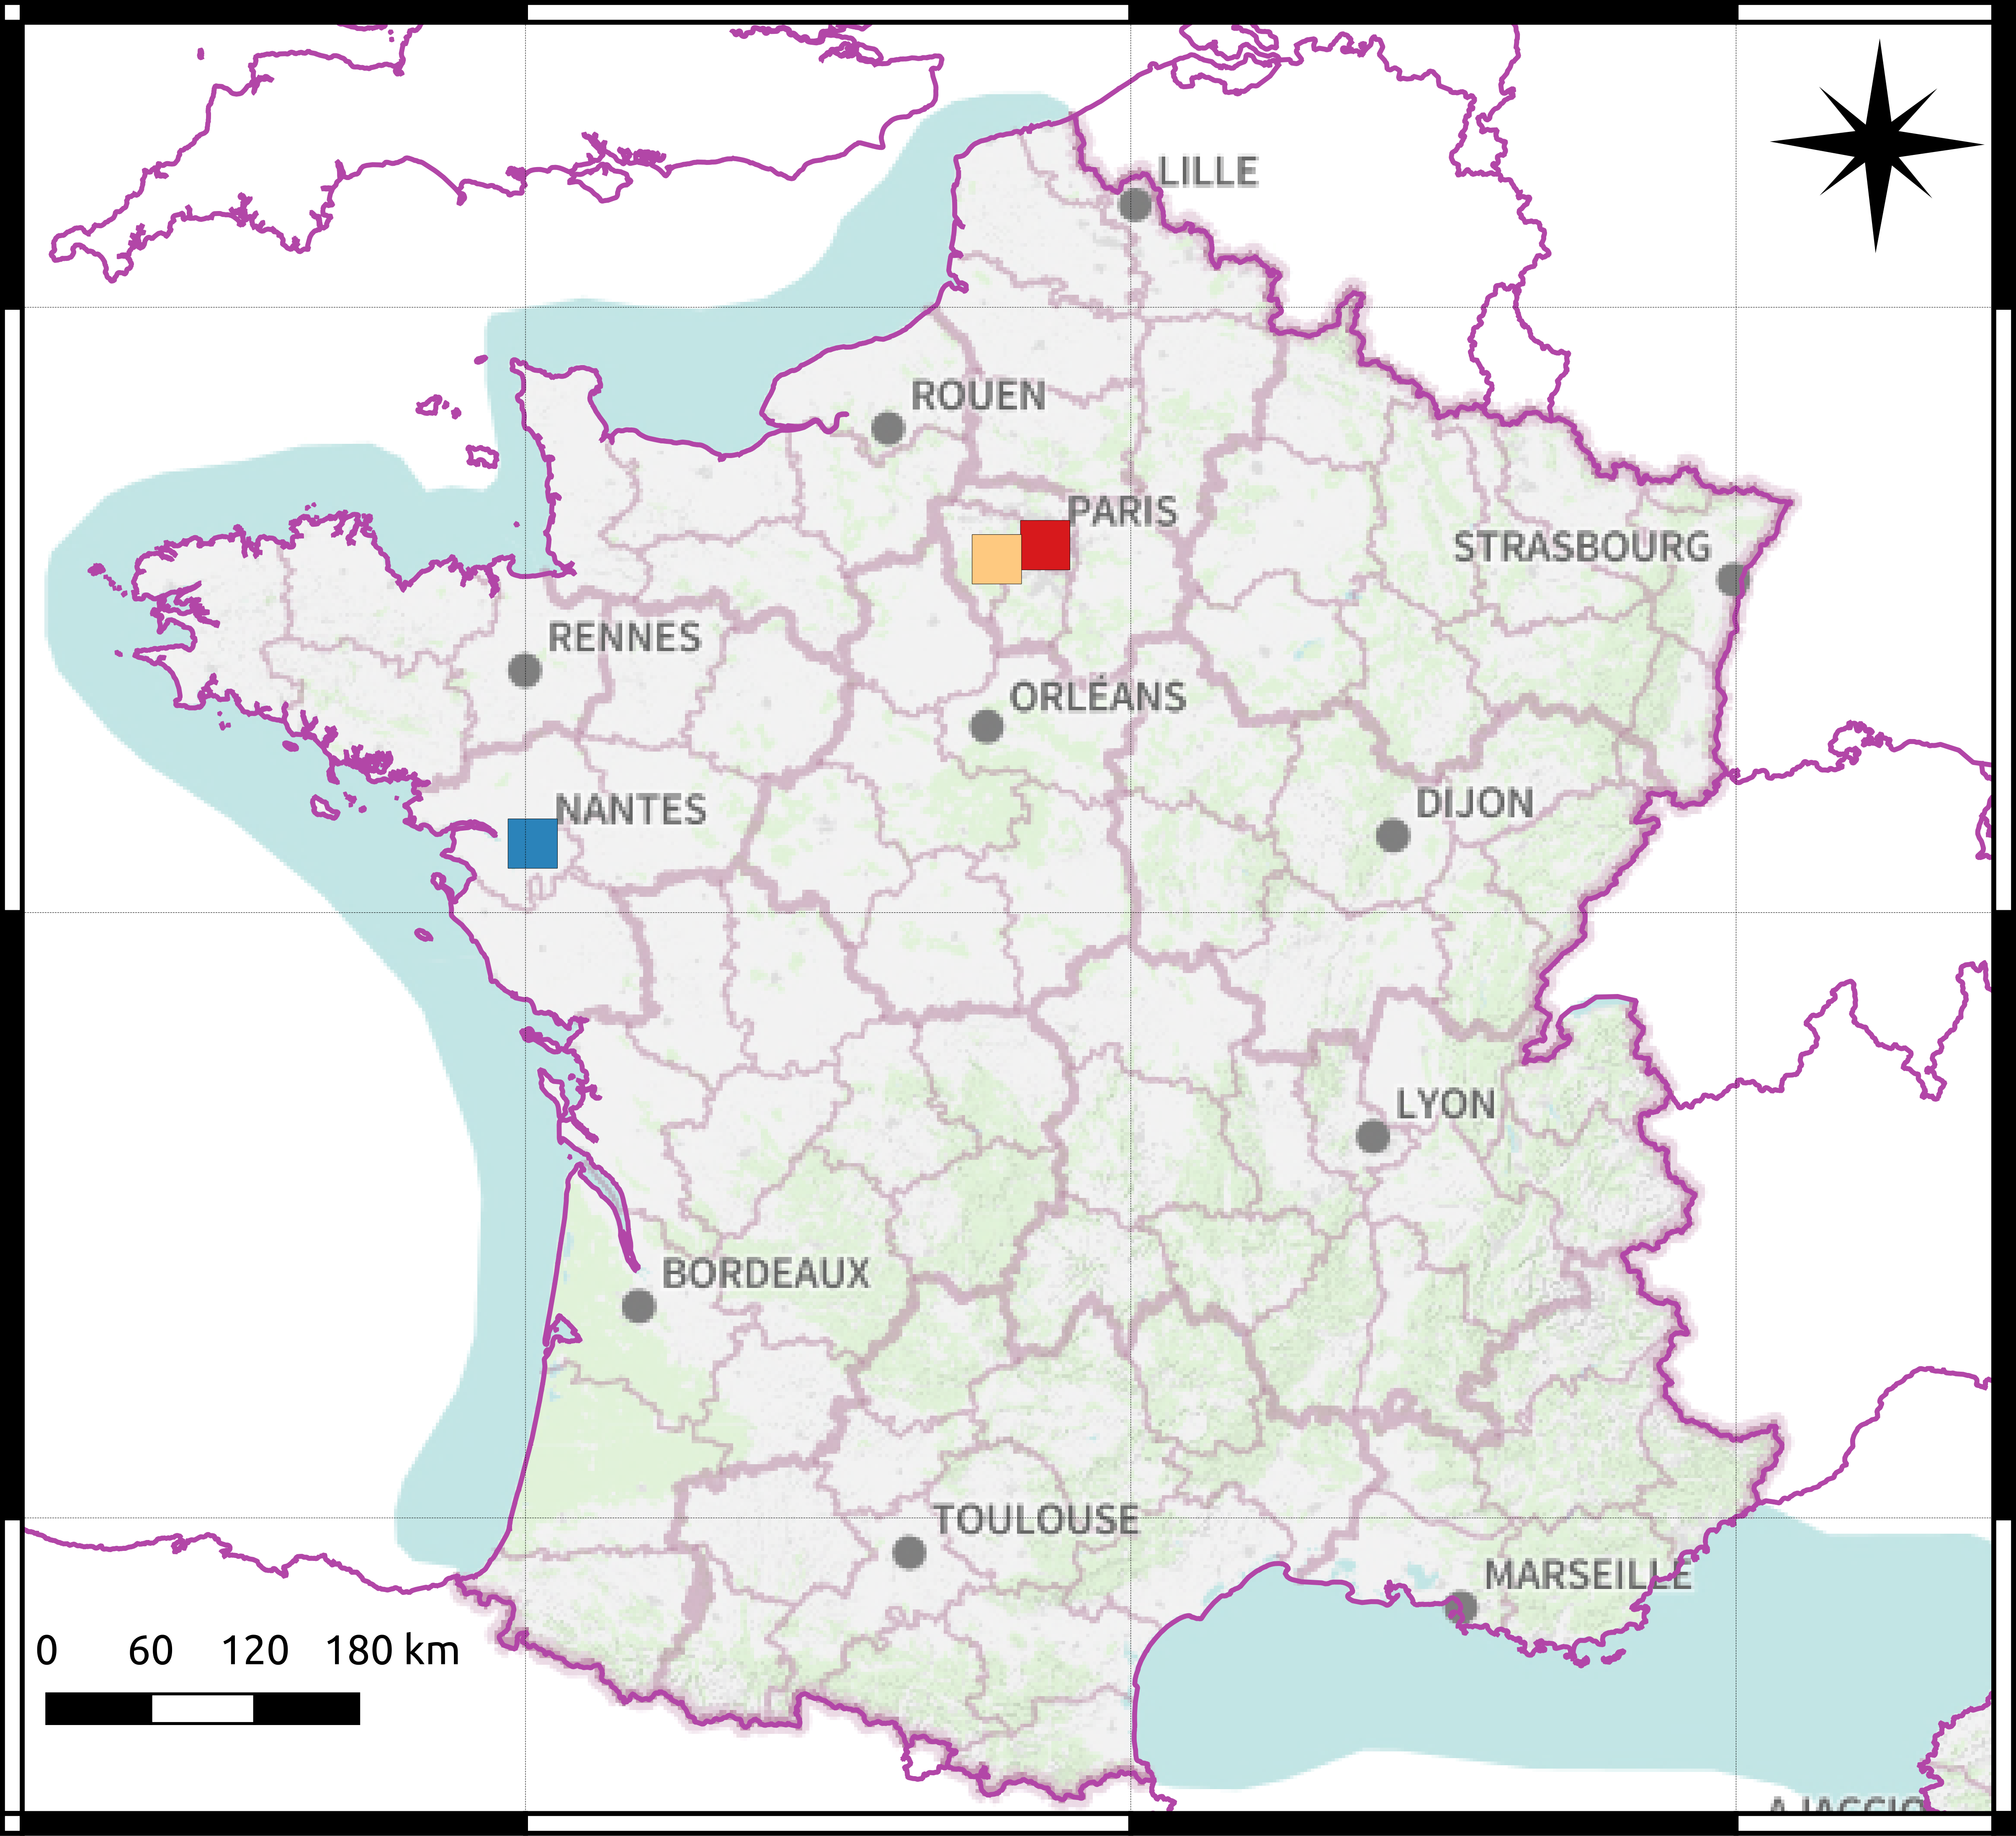
\includegraphics[height=.8\textheight]{images/datasets/france_map}
                }
                \only<2->{
                    \begin{columns}[T]
                        \centering
                        \begin{column}{.48\textwidth}
                            \only<2-4>{
                                \begin{itemize}
                                    \item[\color{elancourt} \(\blacksquare\)]<2-> \textbf{Elancourt}: 
                                        \begin{itemize}[label=\(\blacktriangleright\), font=\color{IGNGreen}]
                                            \item<3-> \num{2009} buildings;
                                            \item<3-> Industrial area;
                                            \item<3-> Residential area;
                                            \item<4-> \gls{acr::dsm} resolution: \SI{0.06}{\m}
                                            \item<4-> Orthoimage resolution: \SI{0.06}{\m}
                                        \end{itemize}
                                \end{itemize}
                            }
                            \only<5-7>{
                                \begin{itemize}
                                    \item[\color{nantes} \(\blacksquare\)]<5-> \textbf{Nantes}: 
                                        \begin{itemize}[label=\(\blacktriangleright\), font=\color{IGNGreen}]
                                            \item<6-> \num{748} buildings;
                                            \item<6-> High buildings;
                                            \item<6-> Dense downtown;
                                            \item<7-> \gls{acr::dsm} res.: \SI{0.1}{\m}
                                            \item<7-> Ortho. res.: \SI{0.1}{\m}
                                        \end{itemize}
                                \end{itemize}
                            }
                            \only<8-10>{
                                \begin{itemize}
                                    \item[\color{paris} \(\blacksquare\)]<8-> \textbf{Paris-13}: 
                                        \begin{itemize}[label=\(\blacktriangleright\), font=\color{IGNGreen}]
                                            \item<9-> \num{478} buildings;
                                            \item<9-> Dense Hausmann style downtown;
                                            \item<9-> Skyscrapers;
                                            \item<10-> \gls{acr::dsm} res.: \SI{0.1}{\m}
                                            \item<10-> Ortho. res.: \SI{0.1}{\m}
                                        \end{itemize}
                                \end{itemize}
                            }
                        \end{column}
                        \begin{column}{.48\textwidth}
                            \begin{overlayarea}{\textwidth}{.8\textheight}
                                \centering
                                \only<2-4>{
                                    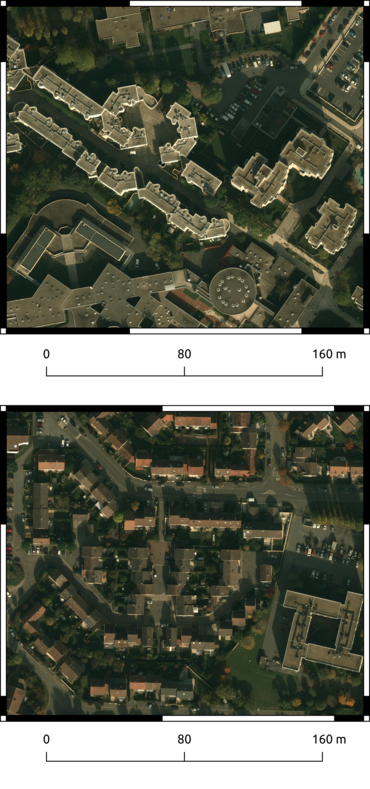
\includegraphics[height=6cm]{images/datasets/elancourt_samples}
                                }
                                \only<5-7>{
                                    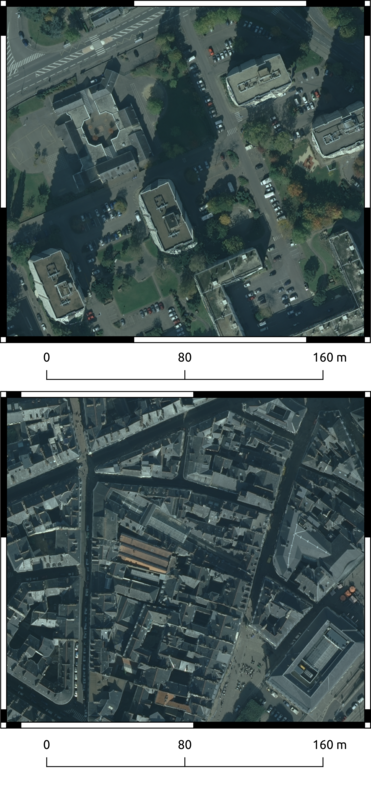
\includegraphics[height=6cm]{images/datasets/nantes_samples}
                                }
                                \only<8-10>{
                                    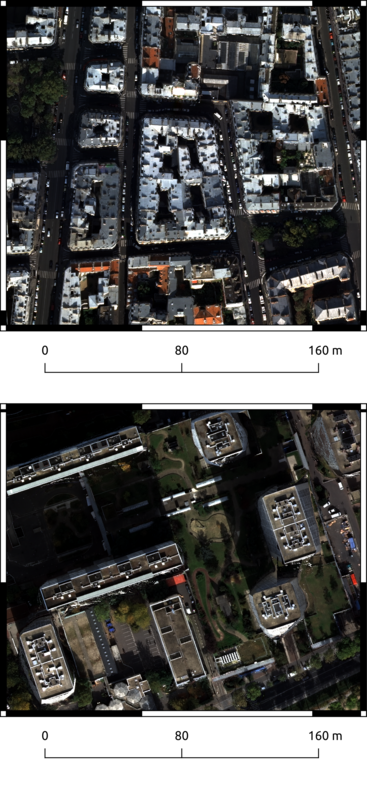
\includegraphics[height=6cm]{images/datasets/paris-13_samples}
                                }
                            \end{overlayarea}
                        \end{column}
                    \end{columns}
                }
            \end{frame}

            \begin{frame}{Annotation procedure}
                \centering
                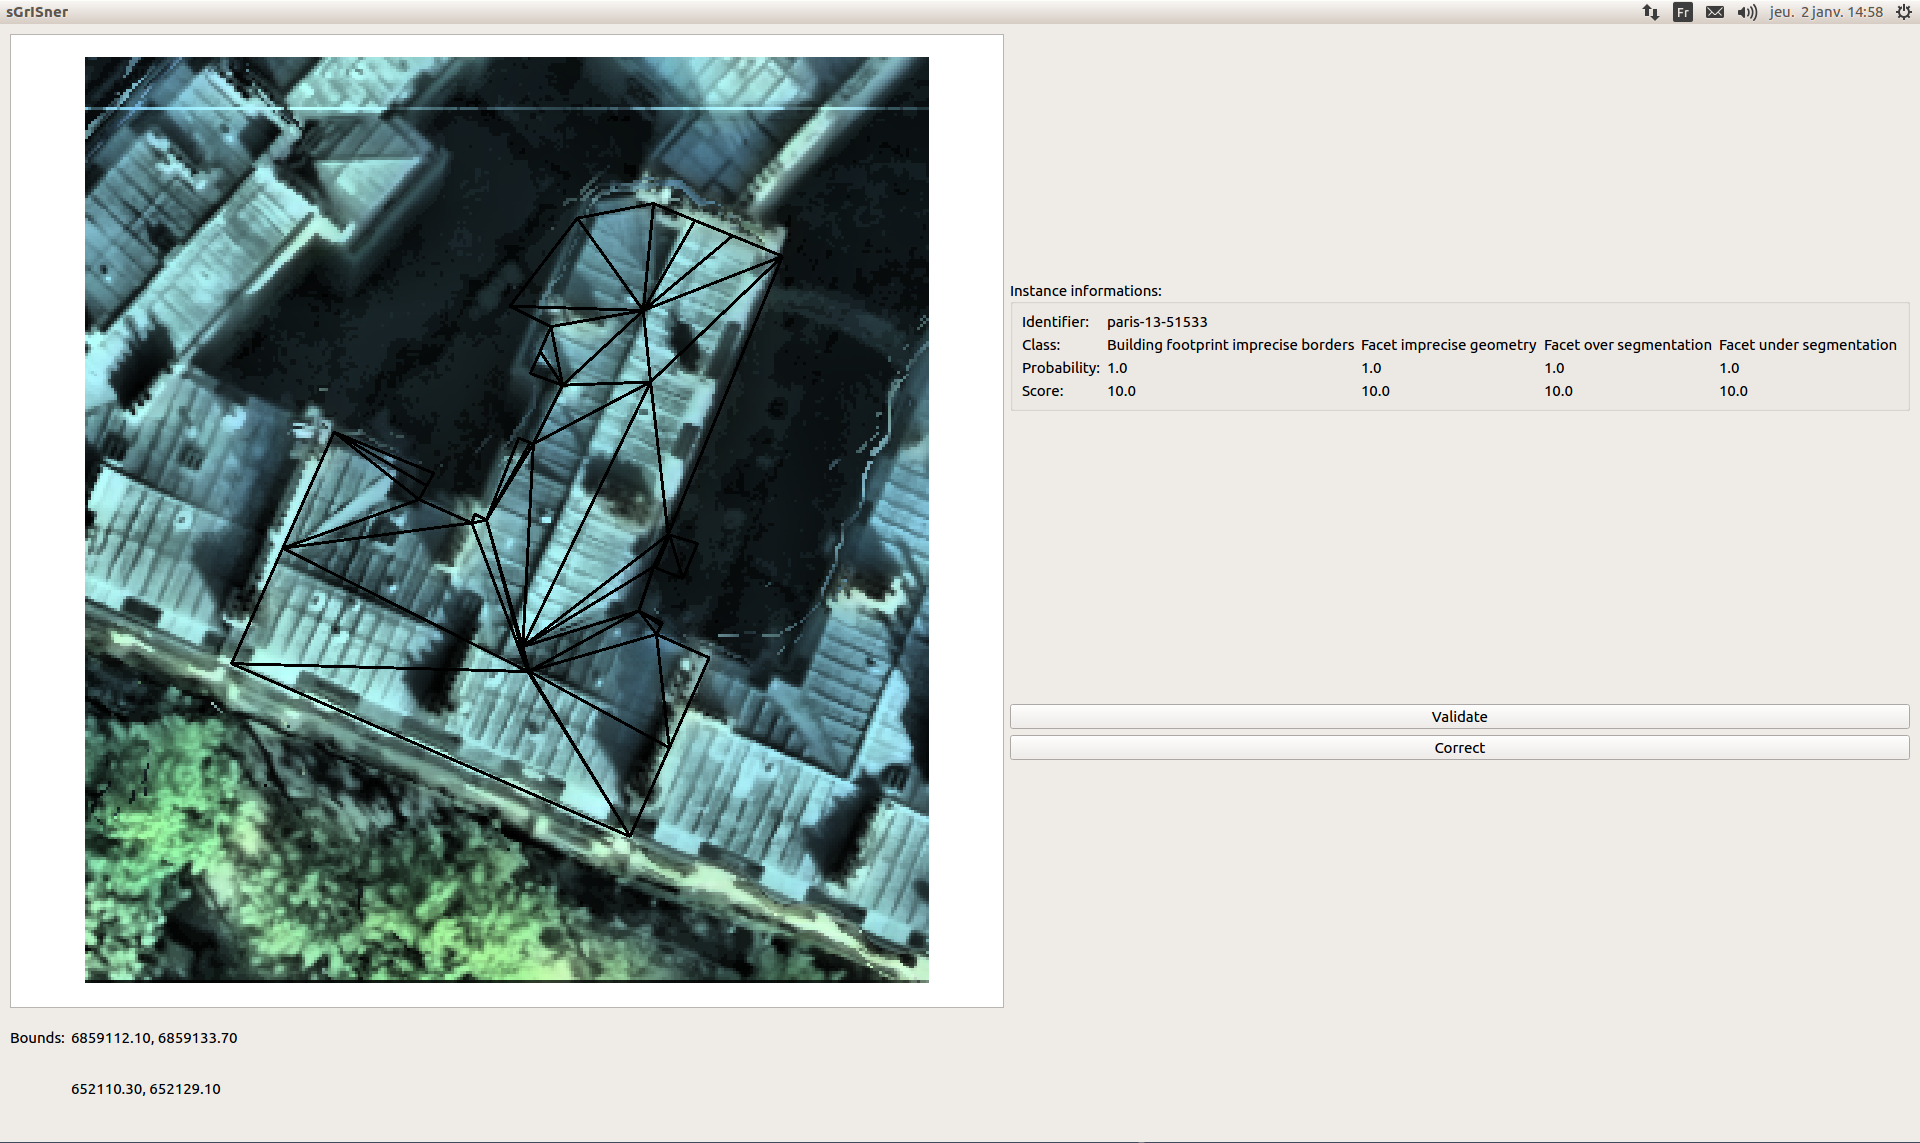
\includegraphics[width=\textwidth]{images/annotations/annotation_rendering}
            \end{frame}

            \begin{frame}{Error statistics}
                \centering
                \only<1>{
                    \includestandalone[mode=buildnew, height=.75\textheight]{figures/datasets/families_stats}
                }
                \only<2>{
                    \includestandalone[mode=buildnew, height=.75\textheight]{figures/datasets/lod1_stats}
                }
                \only<3>{
                    \includestandalone[mode=buildnew, width=\textwidth]{figures/datasets/lod2_stats}
                }
                \only<4->{
                    \begin{itemize}[label=$\blacktriangleright$, font=\color{IGNGreen}]
                        \item<4-> Highly unbalanced data;
                        \item<5-> Dense scenes are comparable;
                        \item<6-> Dense scene:
                        \begin{itemize}[label=\(\implies\)]
                            \item High \texttt{Facet errros} count;
                            \item Low \texttt{Building errros} count;
                        \end{itemize}
                        \item<7-> Sparce scene: inverse.
                    \end{itemize}
                }
            \end{frame}

        \subsection{Setup}
            \begin{frame}{Experiment types}
                \centering
                \includestandalone[mode=buildnew, height=.75\textheight]{figures/scalabitity_graph_animated}
            \end{frame}
            
            \begin{frame}{Parameters}
                \begin{itemize}[label=$\blacktriangleright$, font=\color{IGNGreen}]
                    \item<1-> \Acrfull{acr::rf}:
                    \begin{description}
                        \item<2->[Max depth] \num{4};
                        \item<3->[Number of trees] \num{1000};
                    \end{description}
                    \item<4-> Feature vectors: same length = \num{20}.
                    \item<5-> Feature configurations:
                    \begin{itemize}
                        \item<6-> \textbf{Geom.};
                        \item<7-> \textbf{Geom.} \(\oplus\) \textbf{Hei.};
                        \item<8-> \textbf{Geom.} \(\oplus\) \textbf{Im.};
                        \item<9-> \textbf{All} = \textbf{Geom.} \(\oplus\) \textbf{Hei.} \(\oplus\) \textbf{Im.}.
                    \end{itemize}
                \end{itemize}
            \end{frame}

            \begin{frame}{Possible settings}
                \centering
                \footnotesize
                \begin{tabular}{c c c c c}
                    \toprule
                    Features & Classifier & \textbf{\acrshort{acr::efin}} & Experiment & Number\\
                    \hline
                    \multirow{12}{*}{Baseline} & \multirow{12}{*}{\acrshort{acr::rf}} & \multirow{4}{*}{3} & Vanilla & \cellcolor{IGNGreen}<2-3>{\num{4 x 3}}\\
                    &  &  & Transf. & \cellcolor{IGNGreen}<2-3>{\num{4 x 6}}\\
                    &  &  & Gener. & \cellcolor{IGNGreen}<2>{\num{4 x 3}}\\
                    &  &  & Repres. & \cellcolor{IGNGreen}<2>{\num{4 x 6}}\\
                    \cline{3-5}
                    &  & \multirow{4}{*}{2} & Vanilla & \cellcolor{IGNGreen}<2>{\num{4 x 3}}\\
                    &  &  & Transf. & \cellcolor{IGNGreen}<2>{\num{4 x 6}}\\
                    &  &  & Gener. & \cellcolor{IGNDarkGrey}<2>{\textcolor<2>{white}{\num{4 x 3}}}\\
                    &  &  & Repres. & \cellcolor{IGNGreen}<2>{\num{4 x 6}}\\
                    \cline{3-5}
                    &   & \multirow{4}{*}{1} & Vanilla & \cellcolor{IGNGreen}<2>{\num{4 x 3}}\\
                    &  &  & Transf. & \cellcolor{IGNDarkGrey}<2>{\textcolor<2>{white}{\num{4 x 6}}}\\
                    &  &  & Gener. & \cellcolor{IGNDarkGrey}<2>{\textcolor<2>{white}{\num{4 x 3}}}\\
                    &  &  & Repres. & \cellcolor{IGNDarkGrey}<2>{\textcolor<2>{white}{\num{4 x 6}}}\\
                    \hline
                    \multicolumn{4}{l}{Total} & \num[fraction-function = \sfrac]{144/216}\\
                    \bottomrule
                \end{tabular}
            \end{frame}

        \subsection{Results}
            \begin{frame}{Vanilla experiments}
                \centering
                \only<1>{
                    \includestandalone[mode=buildnew, height=.8\textheight]{figures/results/presentation/vanilla/building}
                }
                \only<2>{
                    \includestandalone[mode=buildnew, height=.8\textheight]{figures/results/presentation/vanilla/facet}
                }
                \only<3->{
                    \begin{itemize}[label=$\blacktriangleright$, font=\color{IGNGreen}]
                        \item<3-> Rare errors are hard to detect \(\longrightarrow\) Use \acrshort{acr::svm}.
                        \item<4-> \texttt{FOS} and \texttt{FIG} are very frequent \(\implies\) easily detected.
                        \item<5-> Geometric features are usually good enough.
                        \item<6-> In general:
                        \begin{itemize}
                            \item<6-> \texttt{Facet errors} better on dense scenes;
                            \item<7-> \texttt{Building errors} better on the space scene;
                        \end{itemize}
                    \end{itemize}
                }
            \end{frame}

            \begin{frame}{Transferability experiments}
                \centering
                \renewcommand{\arraystretch}{1.5}
                \only<1-4>{
                    \footnotesize
                    \centering
                    \begin{tabular}{| c | c | c | c | c |}
                        \hline
                        & \texttt{BOS}  & \texttt{BUS} & \texttt{BIB} & \texttt{BIT} \\
                        \hline
                        \textbf{El.} \(\rightarrow\) \textbf{Na.} & \cellcolor{LOSS1535} & \cellcolor{LOSS1535} \textbf{All} &  & \cellcolor{LOSS0515} \textbf{All} \\
                        \hline
                        \textbf{El.} \(\rightarrow\) \textbf{P13} & \cellcolor{STBL} & \cellcolor{STBL} \textbf{Im.} &  & \cellcolor{STBL} \\
                        \hline
                        \textbf{Na.} \(\rightarrow\) \textbf{P13} & \cellcolor{LOSS1535} & \cellcolor{LOSS1535} \textbf{Im.} &  & \cellcolor{GAIN1535} \textcolor{white}{\textbf{Geom.}} \\
                        \hline
                        \textbf{Na.} \(\rightarrow\) \textbf{El.} & \cellcolor{LOSS0515} & \cellcolor{LOSS1535} \textbf{Im.} & \cellcolor{STBL} \textbf{Im.} & \cellcolor{LOSS1535} \textbf{Geom.} \\
                        \hline
                        \textbf{P13} \(\rightarrow\) \textbf{Na.} & \cellcolor{LOSS0515} & \cellcolor{LOSS1535} \textbf{Im.} &  & \cellcolor{GAIN1535} \textcolor{white}{\textbf{Geom.}} \\
                        \hline
                        \textbf{P13} \(\rightarrow\) \textbf{El.} & \cellcolor{LOSS0515} & \cellcolor{LOSS1535} \textbf{All} & \cellcolor{GAIN0515} \textcolor{white}{\textbf{Im.}} & \cellcolor{LOSS1535} \textbf{Geom.} \\
                        \hline
                    \end{tabular}
                    \vfill
                    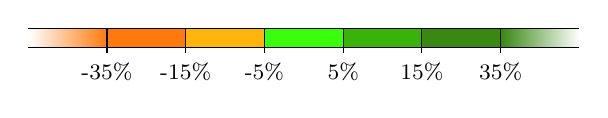
\begin{tikzpicture}
                        \shade[left color=white,right color=LOSS1535] (-1, 0) rectangle (0, .25);
                        \draw[LOSS1535, fill=LOSS1535] (0, 0) rectangle (1, .25);
                        \draw[LOSS0515, fill=LOSS0515] (1, 0) rectangle (2, .25);
                        \draw[STBL, fill=STBL] (2, 0) rectangle (3, .25);
                        \draw[GAIN0515, fill=GAIN0515] (3, 0) rectangle (4, .25);
                        \draw[GAIN1535, fill=GAIN1535] (4, 0) rectangle (5, .25);
                        \shade[left color=GAIN1535,right color=white] (5, 0) rectangle (6, .25);
                        \draw[black] (-1, 0) -- (6, 0);
                        \draw[black] (-1, .25) -- (6, .25);
                        \draw[black] (0, .25) -- (0, -2pt) node[below, black] {\footnotesize -35\%};
                        \draw[black] (1, .25) -- (1, -2pt) node[below, black] {\footnotesize -15\%};
                        \draw[black] (2, .25) -- (2, -2pt) node[below, black] {\footnotesize -5\%};
                        \draw[black] (3, .25) -- (3, -2pt) node[below, black] {\footnotesize 5\%};
                        \draw[black] (4, .25) -- (4, -2pt) node[below, black] {\footnotesize 15\%};
                        \draw[black] (5, .25) -- (5, -2pt) node[below, black] {\footnotesize 35\%};
                    \end{tikzpicture}
                    \uncover<1->{
                        \normalsize
                        \begin{itemize}[label=$\blacktriangleright$, font=\color{IGNGreen}]
                            \item<only@2> Transferability of \texttt{Building errors}: \num[fraction-function = \sfrac]{7/20}.
                            \item<only@3> \texttt{BOS} and \texttt{BUS} are hard to transfer.
                            \item<only@4> External modalities are \underline{critical}.
                        \end{itemize}
                    }
                }
                \only<5-8>{
                    \centering
                    \footnotesize
                    \begin{tabular}{| c | c | c | c | c | c |}
                        \hline
                        & \texttt{FOS} & \texttt{FUS} & \texttt{FIB} & \texttt{FIT} & \texttt{FIG} \\
                        \hline
                        \textbf{El.} \(\rightarrow\) \textbf{Na.} & \cellcolor{STBL} & \cellcolor{LOSS0515} \textbf{Im.} & \cellcolor{LOSS0515} \textbf{Im.} & \cellcolor{GAIN0515} \textbf{Im.} & \cellcolor{STBL} \\
                        \hline
                        \textbf{El.} \(\rightarrow\) \textbf{P13} & \cellcolor{STBL} & \cellcolor{LOSS1535} \textbf{Im.} & \cellcolor{LOSS0515} \textbf{Im.} &  & \cellcolor{STBL} \\
                        \hline
                        \textbf{Na.} \(\rightarrow\) \textbf{P13} & \cellcolor{STBL} & \cellcolor{LOSS1535} \textbf{Geom.} & \cellcolor{STBL} &  & \cellcolor{STBL} \textbf{Hei.} \\
                        \hline
                        \textbf{Na.} \(\rightarrow\) \textbf{El.} & \cellcolor{STBL} & \cellcolor{GAIN0515} \textbf{Im.} & \cellcolor{GAIN1535} \textbf{Im.} & \cellcolor{LOSS0515} & \cellcolor{STBL} \\
                        \hline
                        \textbf{P13} \(\rightarrow\) \textbf{Na.} & \cellcolor{STBL} & \cellcolor{LOSS1535} & \cellcolor{STBL} \textbf{Im.} &  & \cellcolor{STBL} \\
                        \hline
                        \textbf{P13} \(\rightarrow\) \textbf{El.} & \cellcolor{STBL} & \cellcolor{GAIN0515} & \cellcolor{GAIN1535} \textbf{All} & \cellcolor{LOSS0515} & \cellcolor{STBL} \\
                        \hline
                    \end{tabular}
                    \vfill
                    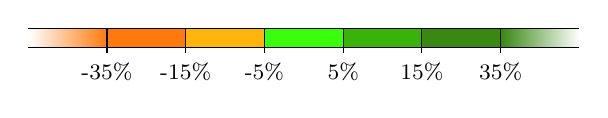
\begin{tikzpicture}
                        \shade[left color=white,right color=LOSS1535] (-1, 0) rectangle (0, .25);
                        \draw[LOSS1535, fill=LOSS1535] (0, 0) rectangle (1, .25);
                        \draw[LOSS0515, fill=LOSS0515] (1, 0) rectangle (2, .25);
                        \draw[STBL, fill=STBL] (2, 0) rectangle (3, .25);
                        \draw[GAIN0515, fill=GAIN0515] (3, 0) rectangle (4, .25);
                        \draw[GAIN1535, fill=GAIN1535] (4, 0) rectangle (5, .25);
                        \shade[left color=GAIN1535,right color=white] (5, 0) rectangle (6, .25);
                        \draw[black] (-1, 0) -- (6, 0);
                        \draw[black] (-1, .25) -- (6, .25);
                        \draw[black] (0, .25) -- (0, -2pt) node[below, black] {\footnotesize -35\%};
                        \draw[black] (1, .25) -- (1, -2pt) node[below, black] {\footnotesize -15\%};
                        \draw[black] (2, .25) -- (2, -2pt) node[below, black] {\footnotesize -5\%};
                        \draw[black] (3, .25) -- (3, -2pt) node[below, black] {\footnotesize 5\%};
                        \draw[black] (4, .25) -- (4, -2pt) node[below, black] {\footnotesize 15\%};
                        \draw[black] (5, .25) -- (5, -2pt) node[below, black] {\footnotesize 35\%};
                    \end{tikzpicture}
                    \uncover<6->{
                        \normalsize
                        \begin{itemize}[label=$\blacktriangleright$, font=\color{IGNGreen}]
                            \item<only@6> Transferability of \texttt{Facets errors}: \num[fraction-function = \sfrac]{20/27}.
                            \item<only@7> Dense scenes are better for \texttt{Facet errors}.
                            \item<only@8> External modalities are \underline{critical}.
                        \end{itemize}
                    }
                }
                \renewcommand{\arraystretch}{1}
                \only<9->{
                    \begin{itemize}[label=$\blacktriangleright$, font=\color{IGNGreen}]
                        \item<9-> \texttt{Facets errors} > \texttt{Building errors}
                        \item<10-> \texttt{BOS} and \texttt{BUS} are hard to transfer.
                        \item<11-> Dense scenes: same behaviour.
                        \item<12-> Dense scenes: better for \texttt{Facet errors}.
                        \item<13-> External modalities are \underline{critical}.
                    \end{itemize}
                }
            \end{frame}
    
    \section{Advanced features}
        \subsection{Advanced graph features}
            \begin{frame}{Our needs}
                \begin{itemize}[label=$\blacktriangleright$, font=\color{IGNGreen}]
                    \item<1-> Global feature for each graph.
                    \item<2-> Take structure into account.
                    \item<3-> Different node attributes: different dynamics.
                    \item<4-> Different building types \(\implies\) different graph sizes.
                    \item<5-> Handle small dataset.
                \end{itemize}                
            \end{frame}

            \begin{frame}{Our solution}
                \begin{itemize}[label=$\blacktriangleright$, font=\color{IGNGreen}]
                    \item<1-> Use kernel trick:
                    \item<2-> Compare graphs with kernels;
                    \item<3-> Instead of computing feature vectors.
                \end{itemize}
            \end{frame}

            \begin{frame}{Graph kernels}
                \centering
                \includestandalone[mode=buildnew, width=\textwidth]{figures/features/graph_kernels/kernels_menu_all}
            \end{frame}

            \begin{frame}{Advanced graph features}
                \raggedleft
                \includestandalone[mode=buildnew, height=.8\textheight]{figures/features/geometric_kernels_animated}
            \end{frame}
    
        \subsection{Advanced image features}
            \begin{frame}{Our needs}
                \begin{itemize}[label=$\blacktriangleright$, font=\color{IGNGreen}]
                    \item<1-> Global feature for an image.
                    \item<2-> Handle both \glspl{acr::dsm} and images.
                    \item<3-> Handle edges.
                    \item<4-> Handle textures.
                    \item<5-> Handle small dataset.
                \end{itemize}
            \end{frame}
            \begin{frame}{\texorpdfstring{\acrshort*{acr::scatnet}}{ScatNet}}
                \begin{itemize}[label=\(\blacktriangleright\), font=\color{IGNGreen}]
                    \item<1-> Reverse engineered \acrfull{acr::cnn}~\parencite{mallat2012group};
                    \item<2-> Ingredients: 
                    \begin{itemize}[label=\(\blacktriangleright\), font=\color{IGNGreen}]
                        \item<3-> Band pass filters \(\longrightarrow\) high frequency information~\parencite{sifre2013rotation};
                        \item<4-> Modulus \(\longrightarrow\) non-linearity~\parencite{anden2014deep};
                        \item<5-> Average pooling operator \(\longrightarrow\) local invariance~\parencite{mallat2012group}.
                    \end{itemize}
                \end{itemize}
            \end{frame}
            
            \begin{frame}{\texorpdfstring{\acrshort*{acr::scatnet}}{ScatNet} filters}
                \centering
                \only<1>{
                    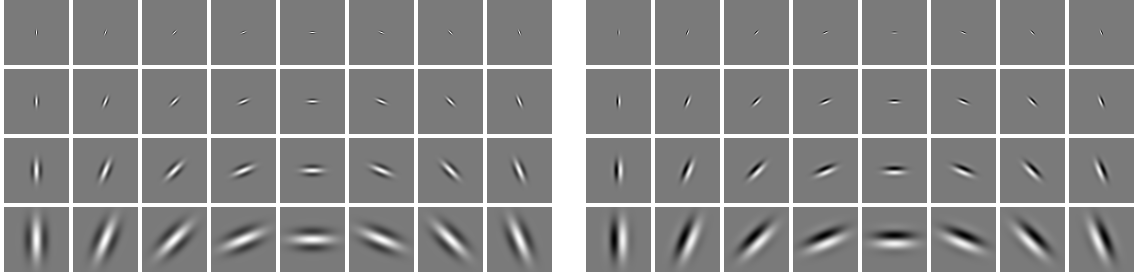
\includegraphics[width=\textwidth]{images/related_work/morlet_wavelets}
                }
                \only<2>{
                    
\includegraphics[width=.35\textwidth]{images/related_work/first_layer_cnn}\\
                    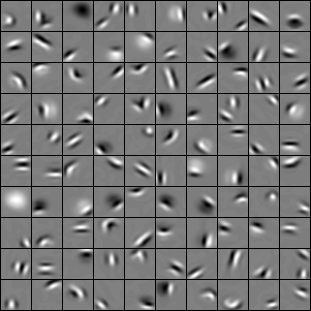
\includegraphics[width=.5\textwidth]{images/related_work/second_layer_cnn}
                }
            \end{frame}

            \begin{frame}{Why using \texorpdfstring{\acrshort*{acr::scatnet}}{ScatNet}}
                \begin{itemize}[label=\(\blacktriangleright\), font=\color{IGNGreen}]
                    \item<1-> Filters are hardcoded not learned:
                    \begin{itemize}
                        \item[\color{IGNDarkGreen} +]<2-> No need for a large dataset;
                        \item[\color{IGNDarkGreen} +]<3-> Interpretable; 
                        \item[\color{red} ---]<4-> Features: not adaptable.
                    \end{itemize}
                    \item<5-> Limited to shallow layers:
                    \begin{itemize}
                        \item[\color{red} ---]<6-> Less powerful~\parencite{oyallon2015deep}.
                    \end{itemize}
                \end{itemize}
            \end{frame}

            \begin{frame}{Advanced height based features}
                \centering
                \includestandalone[mode=buildnew, width=\textwidth]{figures/features/height_based_animated_scatnet}
            \end{frame}

            \begin{frame}{Advanced image based features}
                \centering
                \includestandalone[mode=buildnew, width=\textwidth]{figures/features/image_based_animated_scatnet}
            \end{frame}
        
        \subsection{Experiments}
            \begin{frame}{Possible settings}
                \footnotesize
                \begin{tabular}{c c c c c}
                    \toprule
                    Features & Classifier & \textbf{\acrshort{acr::efin}} & Experiment & Number\\
                    \hline
                    \multirow{2}{*}{Baseline} & \acrshort{acr::rf} & \multirow{6}{*}{3} & \multirow{6}{*}{Vanilla} & \num{4 x 1} \\
                     & \acrshort{acr::svm} &  &  & \num{4 x 2} \\
                    \cline{1-2}
                    \multirow{2}{*}{\gls{acr::scatnet}} & \acrshort{acr::rf} &  &  & \cellcolor{IGNGreen}<2>{\num{6 x 2}} \\
                     & \acrshort{acr::svm} &  &  & \num{6 x 2} \\
                     \cline{1-2}
                    Graph Kernels & \acrshort{acr::svm} &  &  & \num{1 x 2} \\
                    \cline{1-2}
                    GK \(\oplus\) \gls{acr::scatnet} & \acrshort{acr::svm} &  &  & \num{6 x 2} \\
                    \hline
                    \multicolumn{4}{l}{Total} & \num{50}\\
                    \bottomrule
                \end{tabular}
            \end{frame}

            \begin{frame}{Parameters}
                \begin{itemize}[label=$\blacktriangleright$, font=\color{IGNGreen}]
                    \item<1-> \Acrfull{acr::rf}:
                    \begin{description}
                        \item<2->[Max depth] \num{4};
                        \item<3->[Number of trees] \num{1000};
                    \end{description}
                    \item<4-> \gls{acr::scatnet} channel \(\longleftrightarrow\) \num{1085} features
                    \item<5-> Feature configurations:
                    \begin{itemize}
                        \item<6-> \textbf{Geom.};
                        \item<7-> \textbf{Geom.} \(\oplus\) \textbf{S-Hei.};
                        \item<8-> \textbf{Geom.} \(\oplus\) \textbf{S(d)-Im.};
                        \item<8-> \textbf{Geom.} \(\oplus\) \textbf{S(c)-Im.};
                        \item<9-> \textbf{S(d)-All} = \textbf{Geom.} \(\oplus\) \textbf{S-Hei.} \(\oplus\) \textbf{S(d)-Im.}.
                        \item<9-> \textbf{S(c)-All} = \textbf{Geom.} \(\oplus\) \textbf{S-Hei.} \(\oplus\) \textbf{S(c)-Im.}.
                    \end{itemize}
                \end{itemize}
            \end{frame}

            \begin{frame}{\texorpdfstring{\acrshort*{acr::scatnet}}{ScatNet} results}
                \centering
                \small
                \begin{tabular}{| c | c | c | c | c |}
                    \hline
                     & \texttt{BOS} & \texttt{BUS} & \texttt{BIB} & \texttt{BIT} \\
                    \hline
                    \textbf{Elancourt} & \cellcolor{STBL} & \cellcolor{GAIN0515} \textcolor{white}{\textbf{S-Hei.}} & \cellcolor{STBL} & \cellcolor{GAIN1535} \textcolor{white}{\textbf{S-Hei.}} \\
                    \hline
                    \textbf{Na-P13} & \cellcolor{STBL} & \cellcolor{LOSS0515} \textbf{S(d|c)-Im.} & \cellcolor{STBL} & \cellcolor{GAIN0515} \textcolor{white}{\textbf{S(d)-Im.}} \\
                    \hline
                \end{tabular}
                \vfill
                \begin{tabular}{| c | c | c | c | c | c |}
                    \hline
                     & \texttt{FOS} & \texttt{FUS} & \texttt{FIB} & \texttt{FIT} & \texttt{FIG}\\
                    \hline
                    \textbf{Elancourt} & \cellcolor{STBL} & \cellcolor{GAIN1535} \textcolor{white}{\textbf{S(c)-All}} & \cellcolor{GAIN0515} \textcolor{white}{\textbf{S(c)-Im.}} & \cellcolor{GAIN1535} \textcolor{white}{\textbf{S(d)-Im.}} & \cellcolor{GAIN0515} \\
                    \hline
                    \textbf{Na-P13} & \cellcolor{STBL} & \cellcolor{STBL} & \cellcolor{GAIN0515} \textcolor{white}{\textbf{S(c)-Im.}} & \cellcolor{GAIN1535} \textcolor{white}{\textbf{S(c)-Im.}} & \cellcolor{STBL} \\
                    \hline
                \end{tabular}
                \vfill
                \begin{tikzpicture}
                    \shade[left color=white,right color=LOSS0515] (0, 0) rectangle (1, .25);
                    \draw[LOSS0515, fill=LOSS0515] (1, 0) rectangle (2, .25);
                    \draw[STBL, fill=STBL] (2, 0) rectangle (3, .25);
                    \draw[GAIN0515, fill=GAIN0515] (3, 0) rectangle (4, .25);
                    \draw[GAIN1535, fill=GAIN1535] (4, 0) rectangle (5, .25);
                    \shade[left color=GAIN1535,right color=white] (5, 0) rectangle (6, .25);
                    \draw[black] (0, 0) -- (6, 0);
                    \draw[black] (0, .25) -- (6, .25);
                    \draw[black] (1, .25) -- (1, -2pt) node[below, IGNDarkGrey] {\footnotesize -15\%};
                    \draw[black] (2, .25) -- (2, -2pt) node[below, IGNDarkGrey] {\footnotesize -5\%};
                    \draw[black] (3, .25) -- (3, -2pt) node[below, IGNDarkGrey] {\footnotesize 5\%};
                    \draw[black] (4, .25) -- (4, -2pt) node[below, IGNDarkGrey] {\footnotesize 15\%};
                    \draw[black] (5, .25) -- (5, -2pt) node[below, IGNDarkGrey] {\footnotesize 35\%};
                \end{tikzpicture}
                \uncover<2->{
                    \begin{itemize}[label=$\blacktriangleright$, font=\color{IGNGreen}]
                        \item<only@2> Worse only once: \texttt{BUS} on \textbf{Na-P13}.
                        \item<only@3> Better: \num[fraction-function = \sfrac]{9/17}.
                        \item<only@4> External feature helpful for semantic and geometric errors.
                        \item<only@5> Better extractors \(\implies\) external feature more helpful.
                    \end{itemize}
                }
            \end{frame}

            \begin{frame}{Best results}
                \centering
                \only<1>{
                    \includestandalone[mode=buildnew, height=.8\textheight]{figures/results/presentation/best/building}
                }
                \only<2>{
                    \includestandalone[mode=buildnew, height=.8\textheight]{figures/results/presentation/best/facet}
                }
                \only<3->{
                    \begin{itemize}[label=$\blacktriangleright$, font=\color{IGNGreen}]
                        \item<3-> \acrshort{acr::svm} good for highly unbalanced errors.
                        \item<4-> Better feature extractors were beneficial.
                        \item<5-> Only \textbf{Elancourt}: \texttt{Building errors} > \SI{70}{\%}.
                        \item<6-> \texttt{Facet errors} > \SI{70}{\%}.
                    \end{itemize}
                }
            \end{frame}

    \section{Conclusion}
        \begin{frame}{Summary}
            \begin{itemize}[label=\(\blacktriangleright\), font=\color{IGNGreen}]
                \item<1-> \textbf{Hierarchical and modular} error taxonomy;
                \item<2-> \textbf{Scalable} evaluation method;
                \item<4-> Intrinsic features could be used for error prediction;
                \item<5-> Extrinsinc modalities \(\implies\) better transferability.
                \item<6-> Advanced features \(\implies\) high prediction scores.
            \end{itemize}
        \end{frame}
        \begin{frame}{Perspectives}
            \begin{itemize}[label=\(\blacktriangleright\), font=\color{IGNGreen}]
                \item<1-> Use of deep learning:
                \begin{itemize}[label=---]
                    \item Dataset augmentation $\longrightarrow$ \textbf{Simulate errors};
                    \item Semi-supervized learning.
                \end{itemize}
                \item<2-> Localizing errors: facet level.
                \item<3-> Automatic correction.
                \item<4-> Generalize to \gls{acr::lod}-3.
                \item<5-> More modalities: cadastre~\parencite{biljecki2017generating}.
            \end{itemize}
        \end{frame}

    \bgroup
    \setbeamercolor{background canvas}{bg=white}

    \begin{frame}[plain]{}
        \newgeometry{top=0cm, left=0cm, right=0cm, bottom=0cm}
        \hspace{-.75cm}
        \begin{tikzpicture}
            \node (ign_logo) at (-1, 0) {
                
\includegraphics[width=1.606911447cm]{images/logos/logo-ign}
            };
            \path (ign_logo.south) node[anchor=north] (inria_logo) {
                
\includegraphics[width=1.606911447cm]{images/logos/logo-inria}
            };
            \path (inria_logo.south) node[anchor=north] (upe_logo) {
                
\includegraphics[width=1.606911447cm]{images/logos/logo-upe}
            };
            \path (ign_logo.north east) + (3, 0) node[anchor=north west] (trame) {\usebox \tramebox};
            \path (upe_logo.south west) + (0, -1.75) node[anchor=north west] (background) {
                {
                    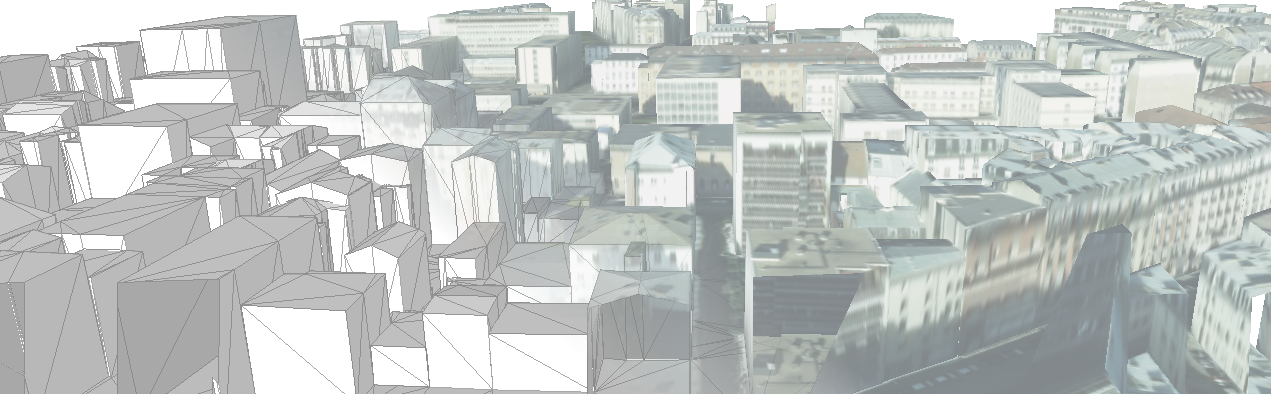
\includegraphics[width=11.5cm]{images/logos/background-50}
                }
            };
            \path (trame.west) + (2.5, -.75) node (title_box) {\usebox \titlebox};
            \path (title_box) + (0, .75) node (thanks) {
                \begin{beamercolorbox}[
                    wd=4cm,
                    sep=8pt
                ]{title page header}
                    \usebeamerfont{title}
                    \begin{center}
                        Thank you for your attention!
                    \end{center}
                \end{beamercolorbox}
            };
            \path (background.north) node[anchor=north] (author) {
                \begin{beamercolorbox}[
                    wd=4cm,
                    sep=8pt
                ]{author}
                    \usebeamerfont{author}
                    \begin{center}
                        \insertauthor\par
                    \end{center}
                \end{beamercolorbox}
            };
            \end{tikzpicture}
        \restoregeometry 
    \end{frame}
    \egroup

    \begin{frame}{Graph kernels}
        \centering
        \includestandalone[mode=buildnew, width=\textwidth]{figures/features/graph_kernels/kernels_menu_all}
    \end{frame}

    \begin{frame}{Random walk on graphs}
        \begin{figure}[H]
            \caption{Random walk on graph \(G\).}
            \alt<1>{
                \centering
                \animategraphics[autoplay, loop, width=.45\textwidth]{25}{figures/features/graph_kernels/drunk_man/drunk_man-}{0}{72}
                \includestandalone[mode=buildnew, width=.45\textwidth]{figures/features/graph_kernels/random_walk}
            }{
                \centering
                \includestandalone[mode=buildnew, width=.45\textwidth]{figures/features/graph_kernels/random_walk}
            }
        \end{figure}
        \begin{itemize}[label=\(\blacktriangleright\), font=\color{IGNGreen}]
            \item<4-> Described \(\longrightarrow\) normalized adjacency matrix \(P\);
            \item<5-> \(P\) as a feature vector \only<6->{ \(\longrightarrow\) \alert<6->{No};}
            \item<7-> \(P\) is not \underline{invariant} to:
            \begin{itemize}[label=-]
                \item<8-> permutations;
                \item<9-> graph size.
            \end{itemize}
            \item<10-> Kernel trick \(\longrightarrow\) compare graphs instead.
        \end{itemize}
    \end{frame}

    \begin{frame}{Random walk based}
        \framesubtitle<1-4>{Random walk kernel}
        \framesubtitle<5-13>{Multiscale Laplacian kernel}
        \framesubtitle<14->{Propagation kernel}
        \only<1-4>{
            \begin{columns}[T]
                \centering
                \begin{column}{.4\textwidth}
                    \centering
                    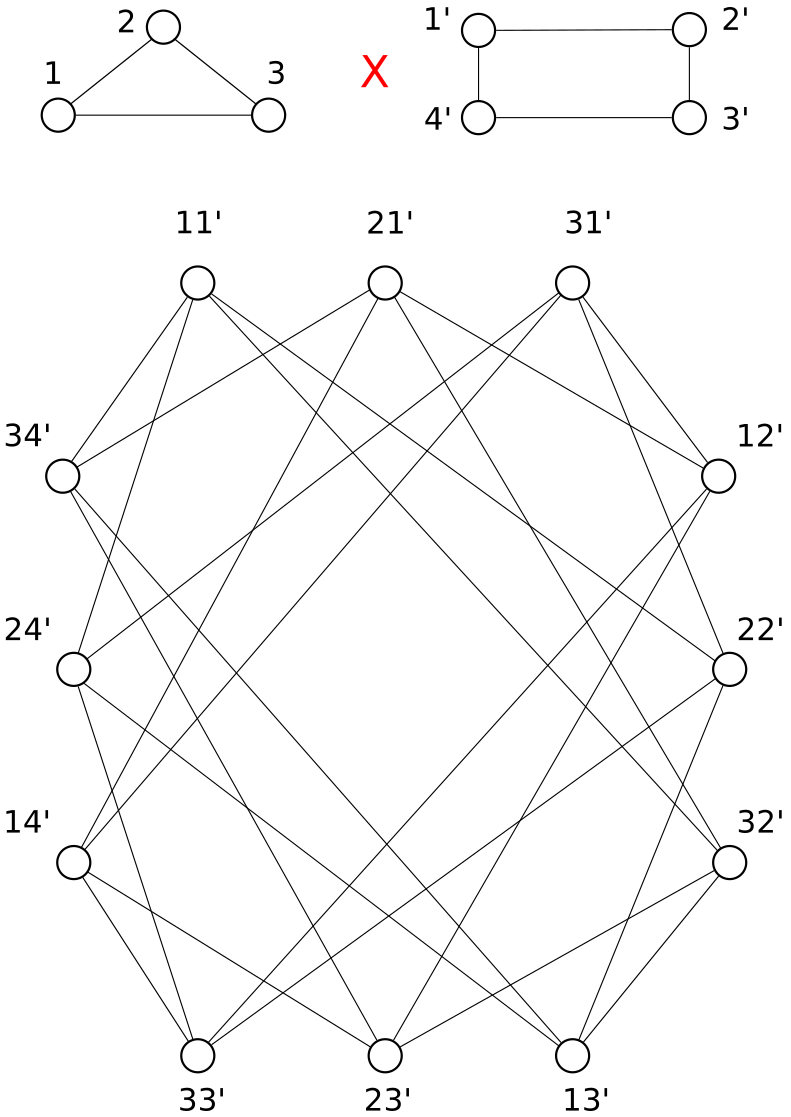
\includegraphics[width=\textwidth]{images/related_work/direct_product_graphs}
                \end{column}
                \begin{column}{.56\textwidth}
                    \centering
                    \begin{itemize}[label=\(\blacktriangleright\), font=\color{IGNGreen}]
                        \item<2-> Quadratic form with \(P_{\times}\) \(\implies\) \underline{invariance} to:
                            \begin{itemize}[label=-]
                                \item<3-> permutation;
                                \item<4-> graph size;
                            \end{itemize}
                    \end{itemize}
                \end{column}
            \end{columns}
        }
        \only<5-13>{
            \vfill
            \begin{itemize}[label=\(\blacktriangleright\), font=\color{IGNGreen}]
                \item<5-> \(G\) \(\longleftrightarrow\) Variance matrix of a \underline{Gaussian distribution}.
                \item<6-> Compare graphs \(\longleftrightarrow\) Compare probabilities.
                \item<7-> Adapted to be:
                \begin{itemize}[label=\(\blacktriangleright\), font=\color{IGNGreen}]
                    \item<8-> permutation and size invariant \(\longrightarrow\) \only<9->{linear embedding;}
                    \item<10-> node attribute aware \(\longrightarrow\) \only<11->{vertex kernel Gram matrix;}
                    \item<12-> scalability \(\longrightarrow\) \only<13->{kernel between pyramid of subgraphs.}
                \end{itemize}
            \end{itemize}
            \vfill
        }
        \only<14->{
            \begin{itemize}[label=\(\blacktriangleright\), font=\color{IGNGreen}]
                \item<14-> Nodes are \underline{Gaussian mixtures} of other nodes;
                \item<15-> Propagate mixture \underline{coefficients} using \(P\);
                \item<16-> Probability distributions are \underline{hashed} \(\longrightarrow\) \onslide<17->{graph feature vector}.
            \end{itemize}
        }
    \end{frame}

    \begin{frame}{Random walk}{Tottering}
        \begin{figure}[H]
            \centering
            \includestandalone[mode=buildnew, width=.5\textwidth]{figures/features/graph_kernels/tottering}
        \end{figure}
        \begin{itemize}
            \item Tottering \(\longleftrightarrow\) cycles;
            \item \textcolor{purple}{Central} nodes are overrepresented;
            \item \textcolor{purple!30}{Isolated} nodes are less visited.
        \end{itemize}
    \end{frame}

    \begin{frame}{Path based}{Graph Hopper kernel}
        \begin{figure}[H]
            \centering
            \includestandalone[mode=buildnew, width=\textwidth]{figures/features/graph_kernels/graph_hopper}
        \end{figure}

        \begin{itemize}[label=\(\blacktriangleright\), font=\color{IGNGreen}]
            \item<2-> Use \underline{paths} instead (no cycles);
            \begin{itemize}[label=\(\blacktriangleright\), font=\color{IGNGreen}]
                \item<3-> Compare same length paths.
                \item<7-> Hop and compare vertex attributes \(\longrightarrow\) base kernel.
                \item<11-> Sum over all vertex comparisons \(\longrightarrow\) \underline{invariance}.
            \end{itemize}
        \end{itemize}
    \end{frame}

    \begin{frame}{Lov\'asz/\texorpdfstring{\acrshort*{acr::svm}}{SVM} kernel}
        \begin{itemize}[label=\(\blacktriangleright\), font=\color{IGNGreen}, itemsep=2em]
            \item<1-> Lov\'asz number \(\vartheta\left(G\right)\):
            \begin{itemize}[label=\(\blacktriangleright\), font=\color{IGNGreen}]
                \item<2-> graph invariant;
                \item<3-> smallest cone containing the orthonormal representation of \(G\).
            \end{itemize}
            \item<4-> Compare graphs \(\longleftrightarrow\) Compare Lov\'asz number of their subgraphs.
            \item<5-> \(\vartheta\left(G\right)\) not easy to compute \(\longleftrightarrow\) Approximation with \gls{acr::svm}kernel.
        \end{itemize}
    \end{frame}


    \begin{frame}{\texorpdfstring{\acrshort*{acr::scatnet}}{ScatNet} structure}
        \centering
        \includestandalone[mode=buildnew, height=.8\textheight]{figures/scattering_network_animated}
    \end{frame}

\end{document}
